\documentclass[a4paper,12pt]{article}
\usepackage{enumerate,amsmath,graphicx,float,epstopdf,subcaption}
\graphicspath{ {./} }
\begin{document}

\title{PHY566 Group Project 1 (A) \\ Random Walk, Diffusion, Cluster Growth}
\date{\small April 3rd, 2015}
\author{David Hicks\\ Weiyao Ke \\ Shagun Maheshwari \\ Fan Zhang}

\maketitle

\section{2D Random Walk}
\subsection{Problem Outline}
In one-dimensional random walk case, let the drunk man move $\pm 1$ in x-coordinate with equal probability at each time-step, repeat this process and average over multiple walkers, the result is the universal law of random walk. Under this condition, the average displacement after numerous steps is expected to be $0$. While the average of squared displacement follows the diffusion equation.
\begin{eqnarray*}
\langle x \rangle &=& 0 \\
\langle x^2 \rangle &=& 2Dt
\end{eqnarray*}
Where, D is diffusion constant for the walk. Then, what will happen to 2D cases? \\

\subsection{Algorithm}
Similar to algorithm of 1D random walk cases, we first generate a random number to decide whether the drunk man will go upwards, leftwards, downwards, or rightwards, with equal probability. Then, repeat this walking process for drunk man for n steps, and average over $10\,000$ drunk men to gain the pattern of average displacement $\langle x \rangle$ and average squared displacement $\langle x^2 \rangle$. \\
In addition, by checking the trend of average squared displacement from origin, we can also calculate the diffusion constant for 2D random walk from function $\langle r^2 \rangle = 2Dt$.

\subsection{Results and Discussion}
\subsubsection{average displacement in x-direction}
After calculating using python, the value of average displacement $\langle x \rangle$ with respect to the number of time-steps n (ranging from $3$ to $100$) is plotted in Fig.~\ref{Fig:xavg}. \\
\begin{figure}[!htb]
  \centering
  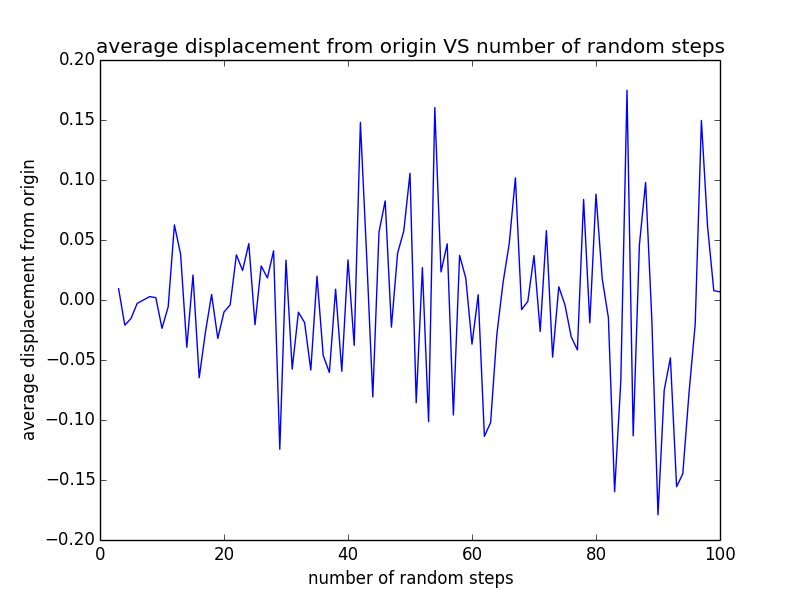
\includegraphics[width=0.6\textwidth]{G:/duke/courses/PHY566/hw6/xavg.png}
  \caption{Average displacement in x-direction with respect to the number of time-steps n.}
  \label{Fig:xavg}
\end{figure}
It could be seen from the graph that, the average displacement fluctuates around the x-axis within a small range ($\pm 0.2$ step). In addition, the larger the number of time-steps, the more the fluctuation is. The pattern of average displacement $\langle x \rangle$ can be concluded to be $$\langle x \rangle \approx 0$$

\subsubsection{average squared displacement in x-direction}
In addition, we also plotted the graph of average squared displacement over number of time-steps n in Fig.~\ref{Fig:x2avg}. \\
\begin{figure}[!htb]
  \centering
  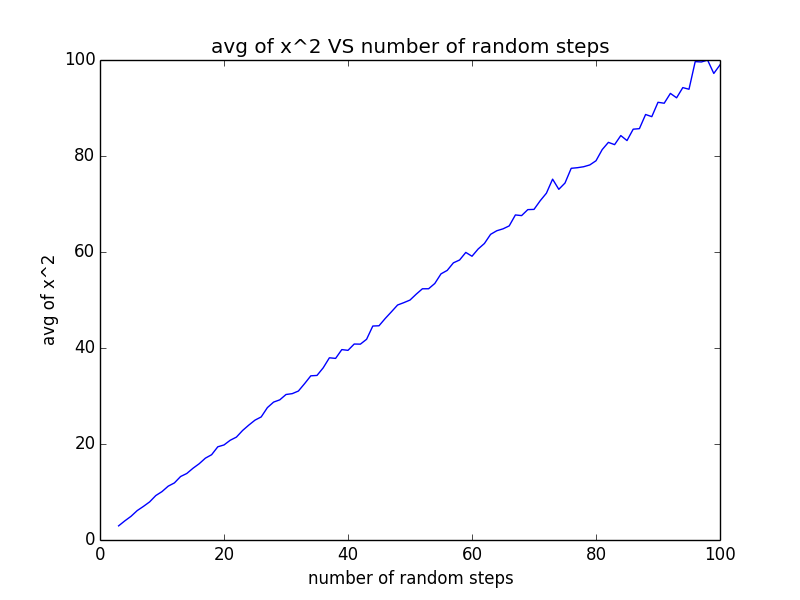
\includegraphics[width=0.6\textwidth]{G:/duke/courses/PHY566/hw6/x2avg.png}
  \caption{Average squared displacement in x-direction with respect to the number of time-steps n.}
  \label{Fig:x2avg}
\end{figure}
In the graph, the average squared displacement in x-direction increases with the number of time-steps n. According to the graph, its linearity can approximately be concluded to be $$\langle x^2 \rangle \approx n$$ Compared to its diffusion equation in x-direction $\langle x^2 \rangle = 2Dt$, the diffusion constant in x-direction is approximately $1/2$.

\subsubsection{average squared displacement from origin}
In this $2$-dimensional case, the random walker's displacement from origin is $r^2 = x^2 + y^2$, it also obeys the diffusion equation. The relationship between average squared displacement from origin and number of time-steps n is plotted in Fig.~\ref{Fig:r2avg}. \\
\begin{figure}[!htb]
  \centering
  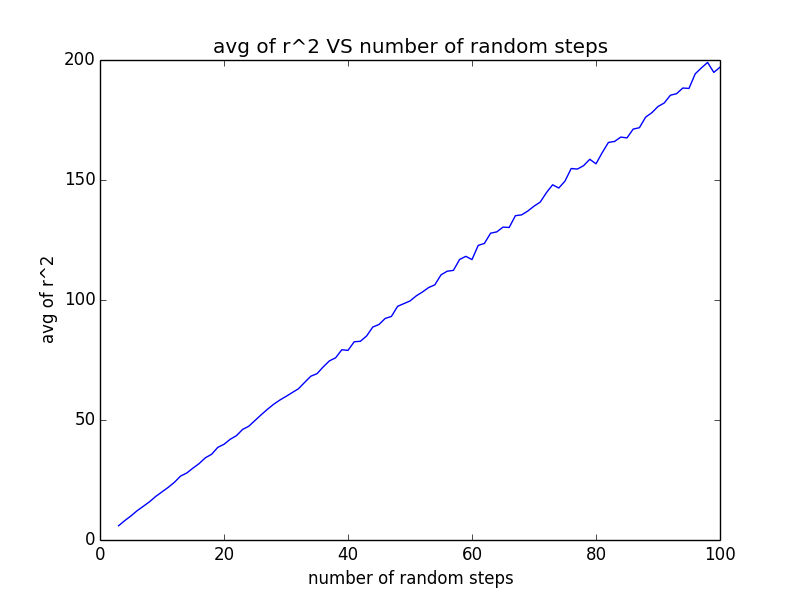
\includegraphics[width=0.6\textwidth]{G:/duke/courses/PHY566/hw6/r2avg.png}
  \caption{Average squared displacement from origin with respect to the number of time-steps n.}
  \label{Fig:r2avg}
\end{figure}
From the plot, the average squared displacement from origin $\langle r^2 \rangle$ increases with the number of time-step n. From eye-measuring, their relationship can be approximated to be $$\langle r^2 \rangle \approx 2n$$ Thus, the diffusion constant for 2D displacement from origin is approximately $1$.


\section{Diffusion Equation}
\subsection{1D diffusion Equation Outline}
\indent
\indent The homogeneous 1D diffusion Equation reads,
\begin{equation}
	\frac{\partial f}{\partial t} = D \nabla^2 f.
\end{equation}
where $D$ is the diffusion constant. For a initial delta distribution $f(x, t = 0) = \delta(x)$, the time evolution of the diffusing density profile is solved by a expanding gaussian wave packet,

\begin{eqnarray*}
	f(x,t) &=& \frac{1}{\sqrt{4\pi D t}} \exp{(-\frac{x^2}{4Dt})}, \\
	f(x, t \rightarrow 0^+) &=& \delta(x).
\end{eqnarray*}

Generally, the expectation value $<x^2(t)>$ at certain time $t$ of a gaussian distribution with a time dependent width $\sigma(t)$ is,
\begin{eqnarray*}
	<x^2(t)> = \int_{-\infty}^{+\infty} x^2 f(x,t) dx &=&  \int_{-\infty}^{\infty}  \frac{1}{\sqrt{2\pi \sigma^2(t)}} x^2 \exp{(-\frac{x^2}{2\sigma^2(t)})} dx, \\
	& = & -\lim_{\beta\rightarrow 1}\frac{d}{d\beta}\int_{-\infty}^{\infty}  \sqrt{\frac{\sigma^2(t)}{\pi}} \exp{(-\beta \frac{x^2}{2\sigma^2(t)})} dx, \\
	& = & -\lim_{\beta\rightarrow 1} 2\sigma^2(t)\frac{d}{d\beta}\sqrt{\beta}, \\
	& = & \sigma^2(t). 
\end{eqnarray*}
As a result, we expect that the root mean square of the solution of the diffusion equation with an delta function like initial configuration grows like $2Dt$ with the time evolution. 

To verify this argument above, we solve the 1D diffusion equation numerically, fit the solution at several time step by gaussian wave packet and extract the time evolution of the root mean square $<x^2>$ as a function of $t$.

\subsection{Algorithm}
To solve the 1D diffusion numerical, we first discretise the partial differential with respect to time and space:
\begin{eqnarray*}
\frac{f_{n+1,i}-f_{n,i}}{\Delta t}  &=& D\frac{f_{n,(i+1)\mod N}+f_{n,(i-1)\mod N} - 2 f_{n,i}}{{\Delta x}^2},\\
t &=& n \Delta t, \\
x &=& i \Delta x.
\end{eqnarray*}
$N$ is the number of spatial grids, the $\mod$ function imposes a periodic boundary condition of the problem, which is equivalent to solve the diffusion equation on a 1D ring.

This is then cast into a time evolution form of a time iteration:
\begin{eqnarray*}
f_{n+1,i} &=&  (1 - 2 \alpha) f_{n,i} + \alpha (f_{n, (i+1)\mod N}+f_{n, (i-1)\mod N}), \alpha = \frac{D\Delta t}{{\Delta x}^2},\\
f_{0,j} &=& f_0(j\Delta x).
\end{eqnarray*}
where $f_0$ is the initial density distribution. Here we set $f_0$ zero except for a short interval resembling a delta function initial condition. The stability criterion for this method is given by $\alpha < 1/2$. This condition is always checked ahead of calling the solver. 

\subsection{Results and Discussion}
\begin{figure}[htbp]
\begin{center}
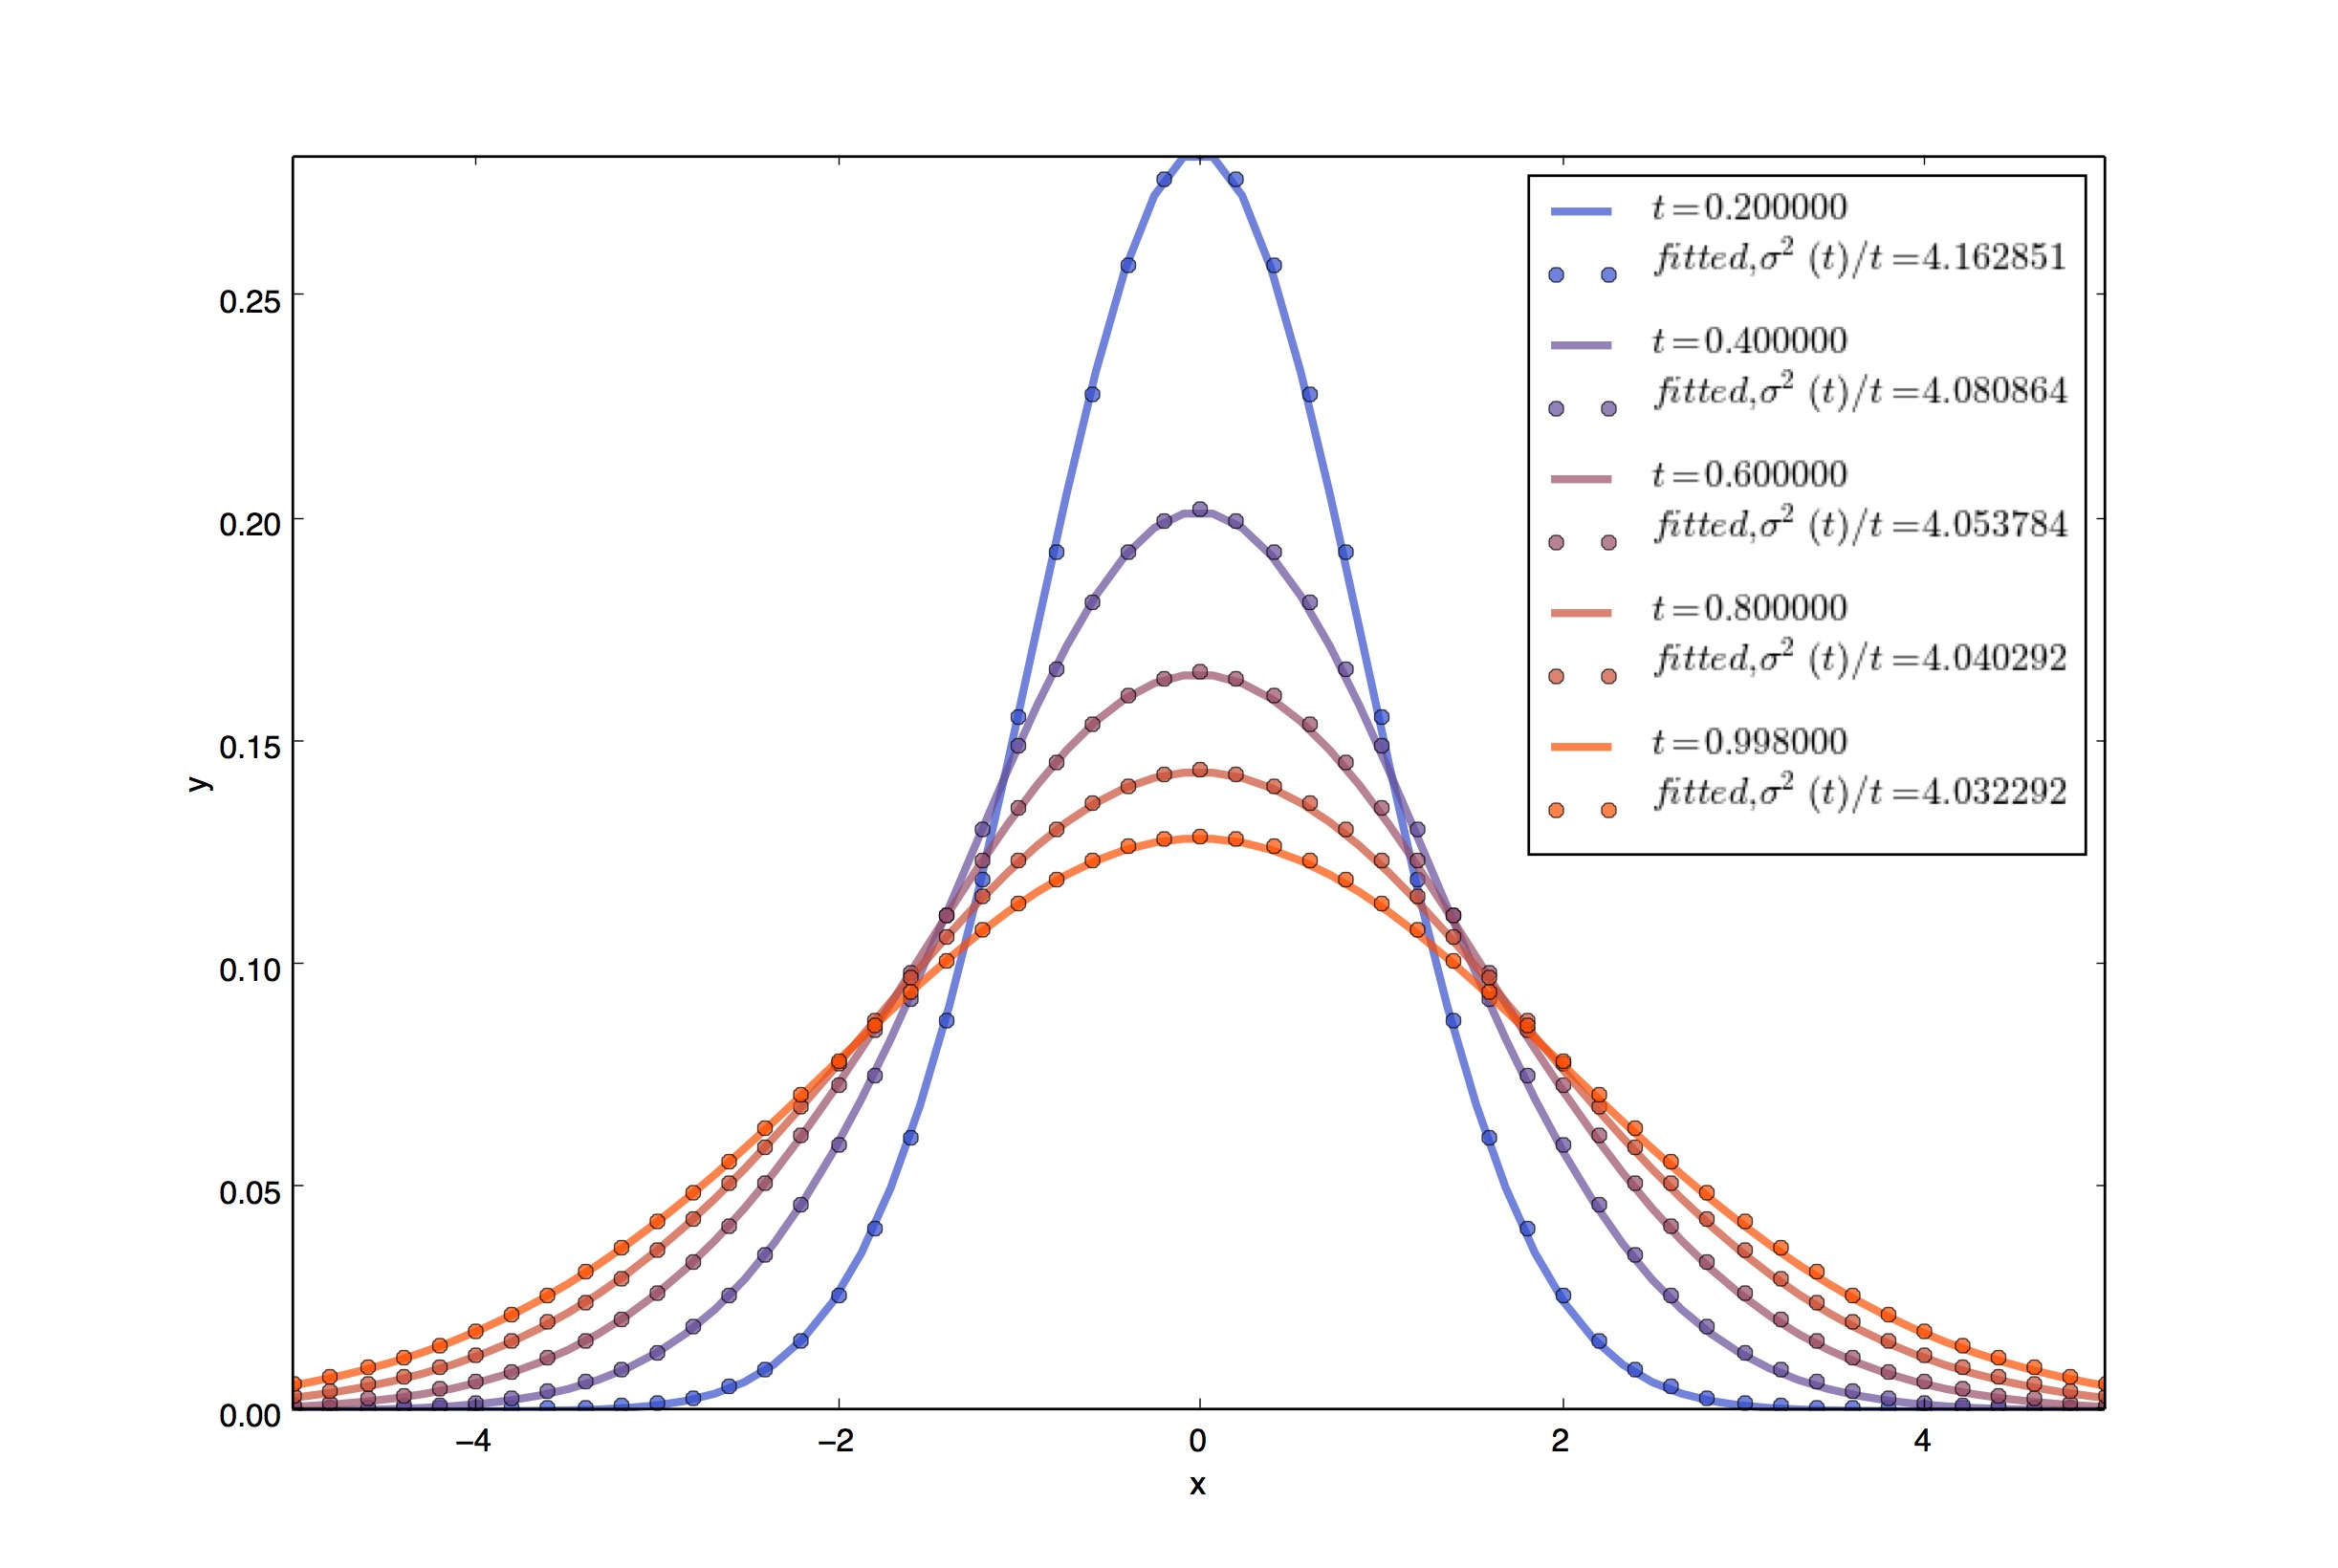
\includegraphics[width = \textwidth]{pics/diffusion_snapshot.jpeg}
\caption{Five snapshots at $t = 0.2, 0.4, 0.6, 0.8, 1.0 t_{max}$. Solid curve is the calculated density profile; solid dots are gaussian fitting results with the quantity $\sigma(t)^2/t$ displayed. It can be seen that the ration $\sigma(t)^2/t$ approach the limit $2D = 4$ with the time evolution and it is almost a constant of time.}
\label{default}
\end{center}
\end{figure}



\section{Cluster Growth with the DLA Model}
\subsection{Problem Outline}
\indent
\indent The random walk concept can also be used to model cluster growth.  In particular, there are two common types of cluster growth methods involving random walks.
The first is known as the Eden Model.  In the Eden model, a seed particle is place in the center of our system and the all of the perimeter sites are identified.  The 
random walk concept is used to randomly choose at which perimeter site a particle will be added.  This is process continues until the desired cluster size is attained.
In this method, the cluster is typically compact with a few number of holes due to the nature of this growth model.  The Eden model grows clusters from the "center-out" 
and is referred to as a "cancer model". 

\indent The other common cluster growth is the diffusion limited aggregation (DLA) model.  Similar to the Eden model, the DLA model starts with a seep particle at 
the center of our system; however, the added particle is randomly generated at a certain distance from the center of the system.  The particle must then perform 
numerous random walks until the particle hits one of the perimeter sites of the central cluster.  The perimeter sites are updated and the procedure continues until
the cluster is a specified size.  In contrast to the Eden model, the DLA model clusters are often extremely sparse and consist of many branches stemming from the 
central cluster.

\subsection{Solution}
\indent
\indent The growth of a cluster was simulated using the DLA model.  The proposed radius of the system is about 100 units.  A seed particle was placed in the center of 
the system and for each iteration the intial position of a random walker at a radius of 100 was generated.  The random walk of this walker was determined using a 
random number generator.  The directions up, down, left, and right were chosen depending on the random number between 0 and 1 (see Python code). The walker's random path
continued until it hit the cluster's perimeter or until it traveled a certain radius away from the cluster.  If the walker traveled a certain distance away from the 
cluster then the walker is said to not return to the cluster in a sufficiently short amount of time, so the walker is thrown out and a new one is generated.

\indent The aformentioned procedure was carried out until the desired radius of 100 units was obtained.  A total of 10 clusters were grown using the DLA method.  The
results are shown in the next section.

\begin{figure}[htbp]
\begin{center}
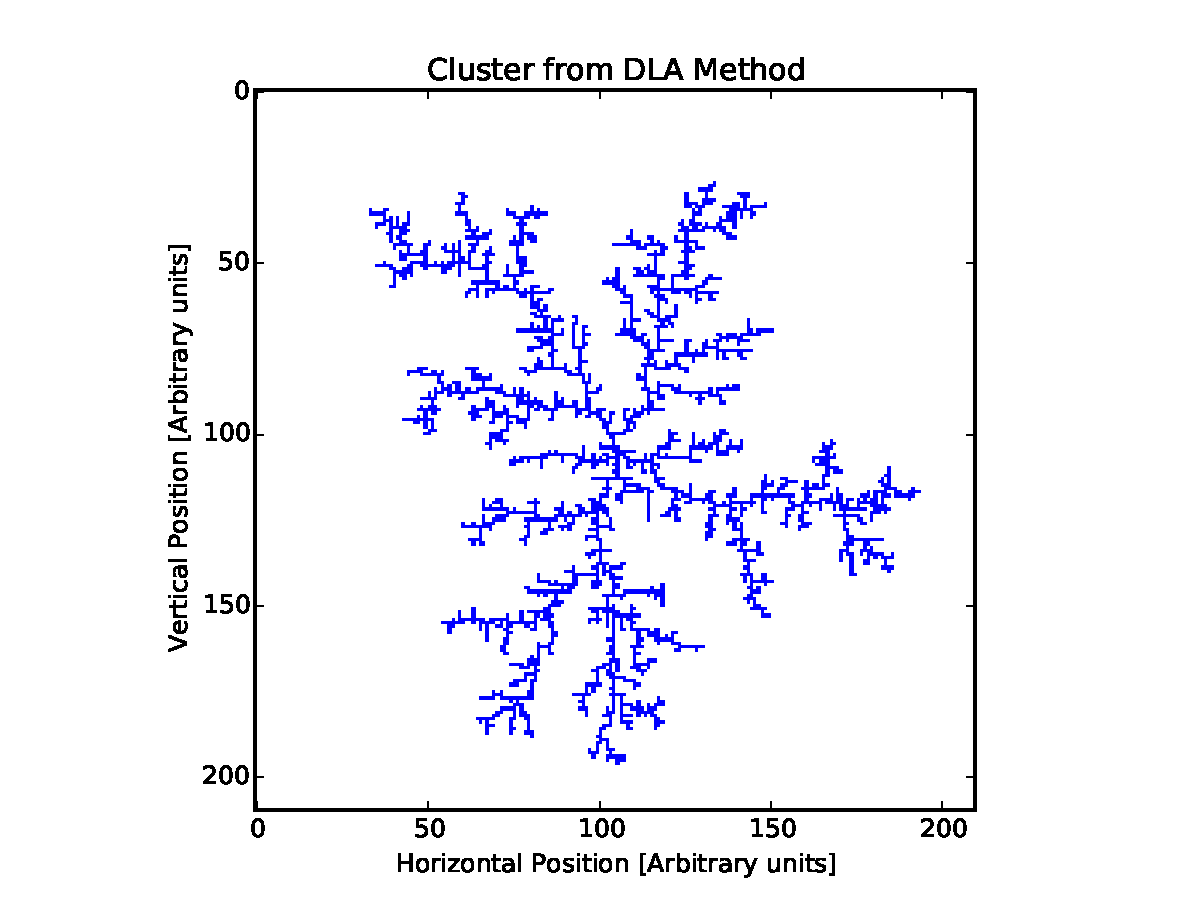
\includegraphics[width = \textwidth]{pics/DLA_crystal_final_1.pdf}
\caption{DLA cluster: Trial 1. The number of walkers used was ....}
\label{DLAcluster1}
\end{center}
\end{figure}

\begin{figure}[htb]
\centering
	\begin{tabular}{@{}cc@{}}
		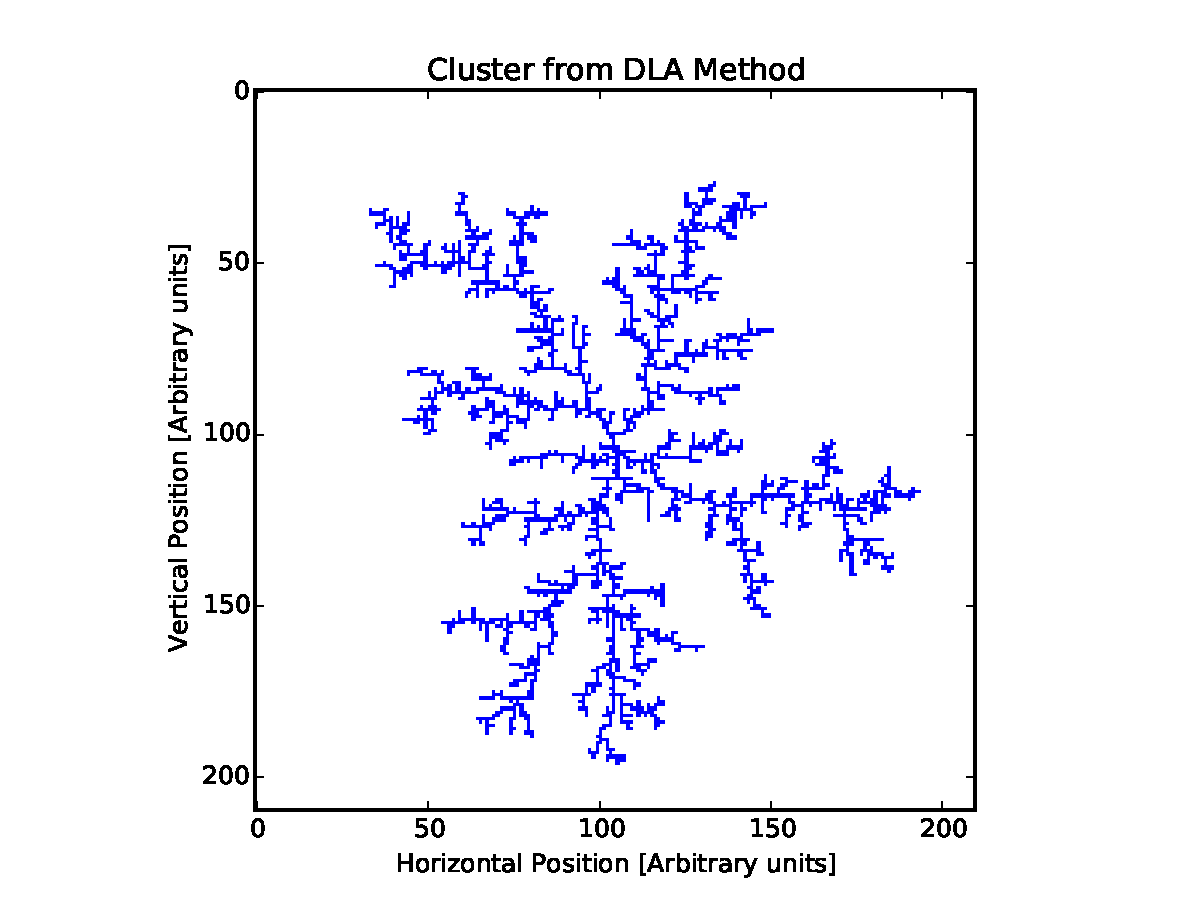
\includegraphics[width = 0.45\textwidth]{pics/DLA_crystal_final_1.pdf} &
		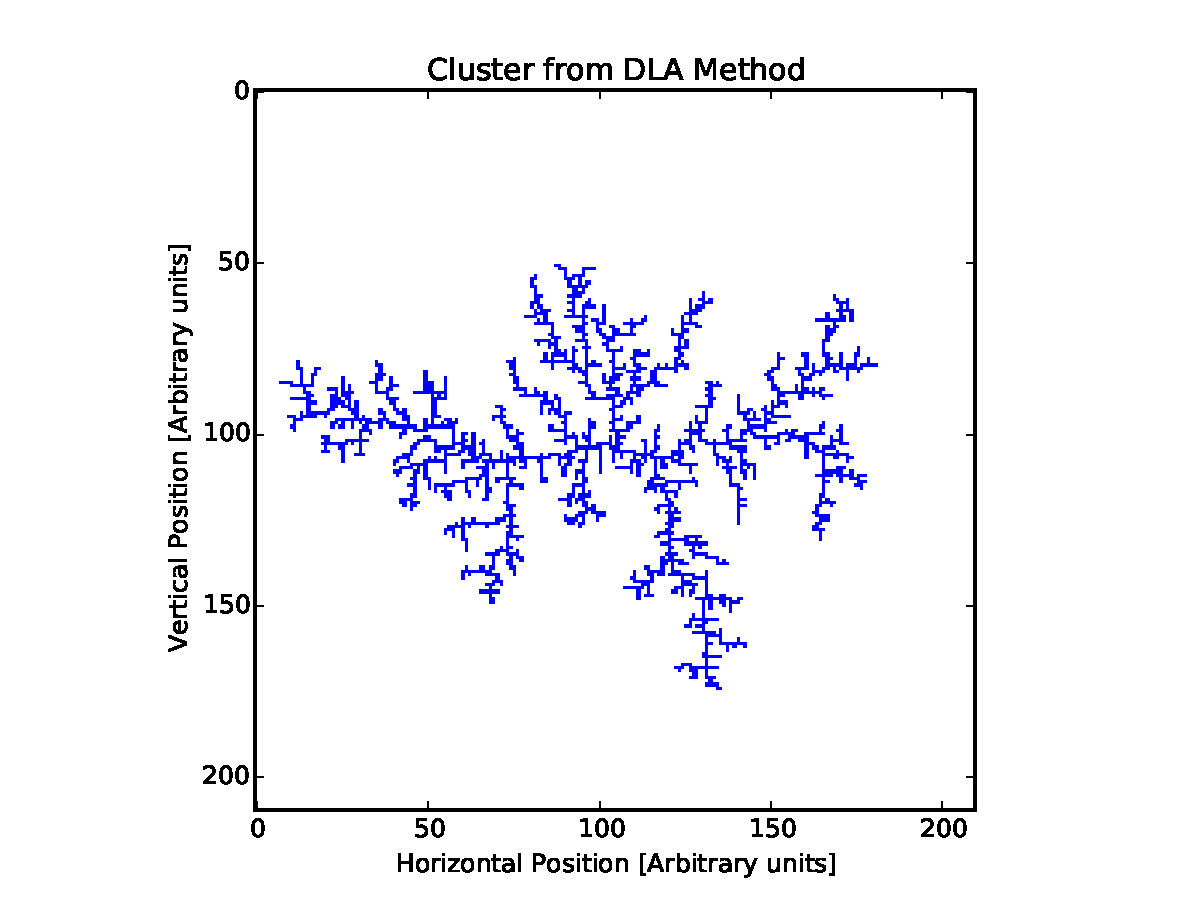
\includegraphics[width = 0.45\textwidth]{pics/DLA_crystal_final_2.pdf} \\
		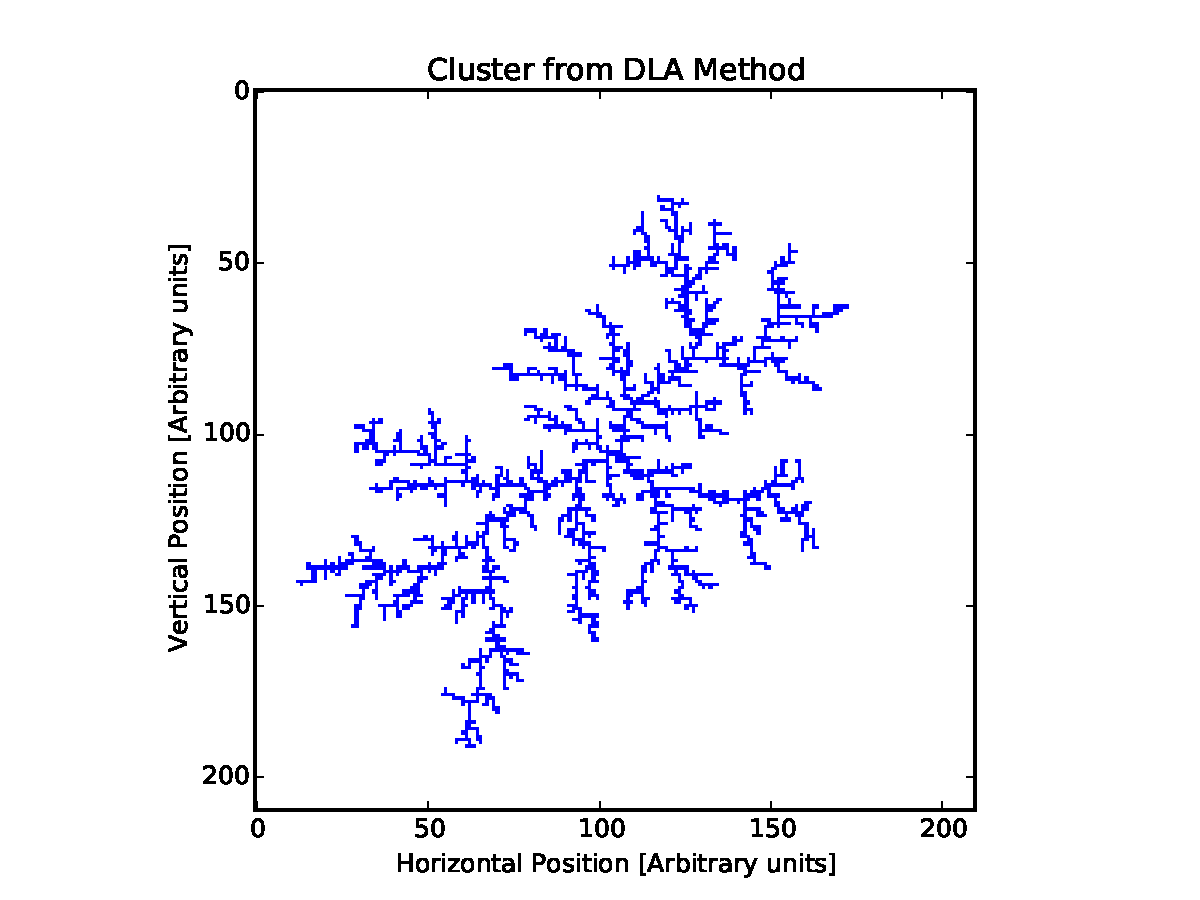
\includegraphics[width = 0.45\textwidth]{pics/DLA_crystal_final_3.pdf} &
		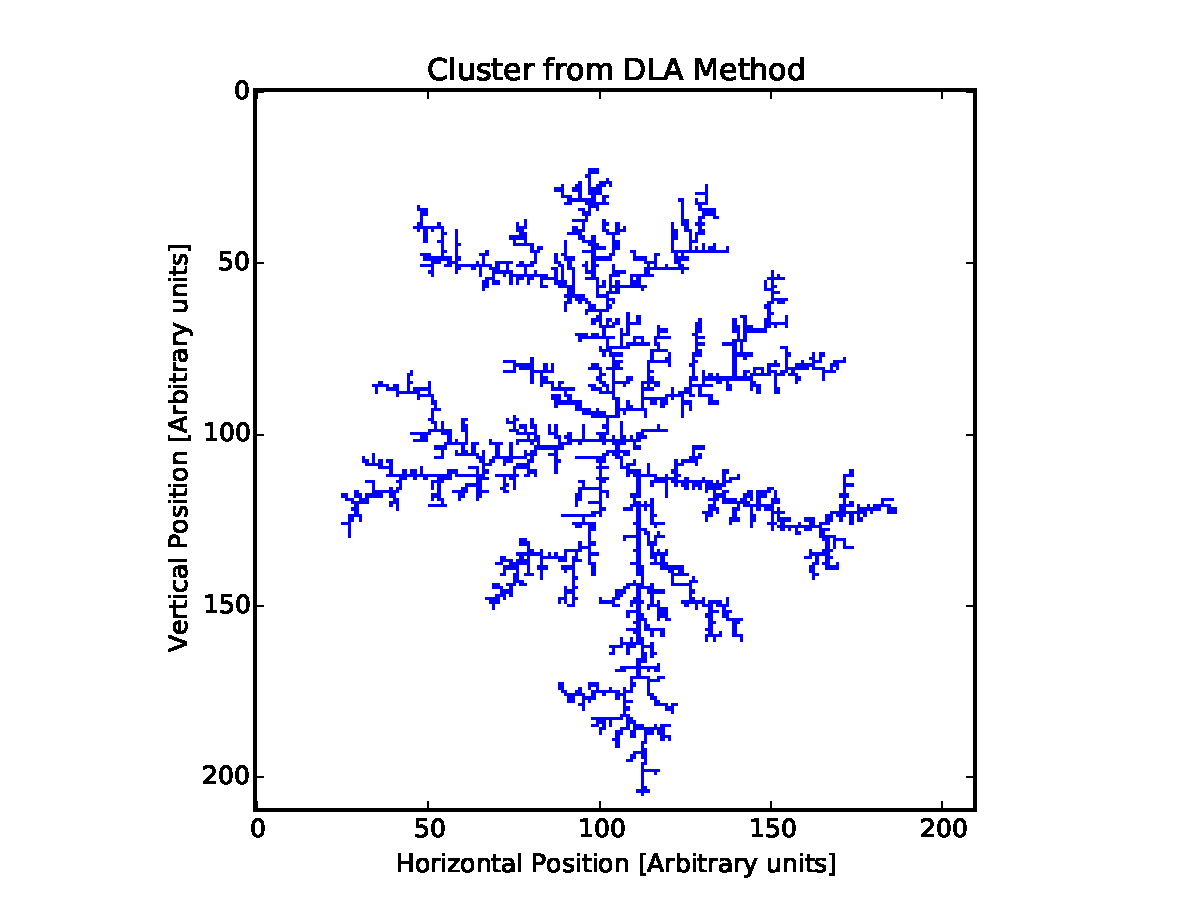
\includegraphics[width = 0.45\textwidth]{pics/DLA_crystal_final_4.pdf} \\
		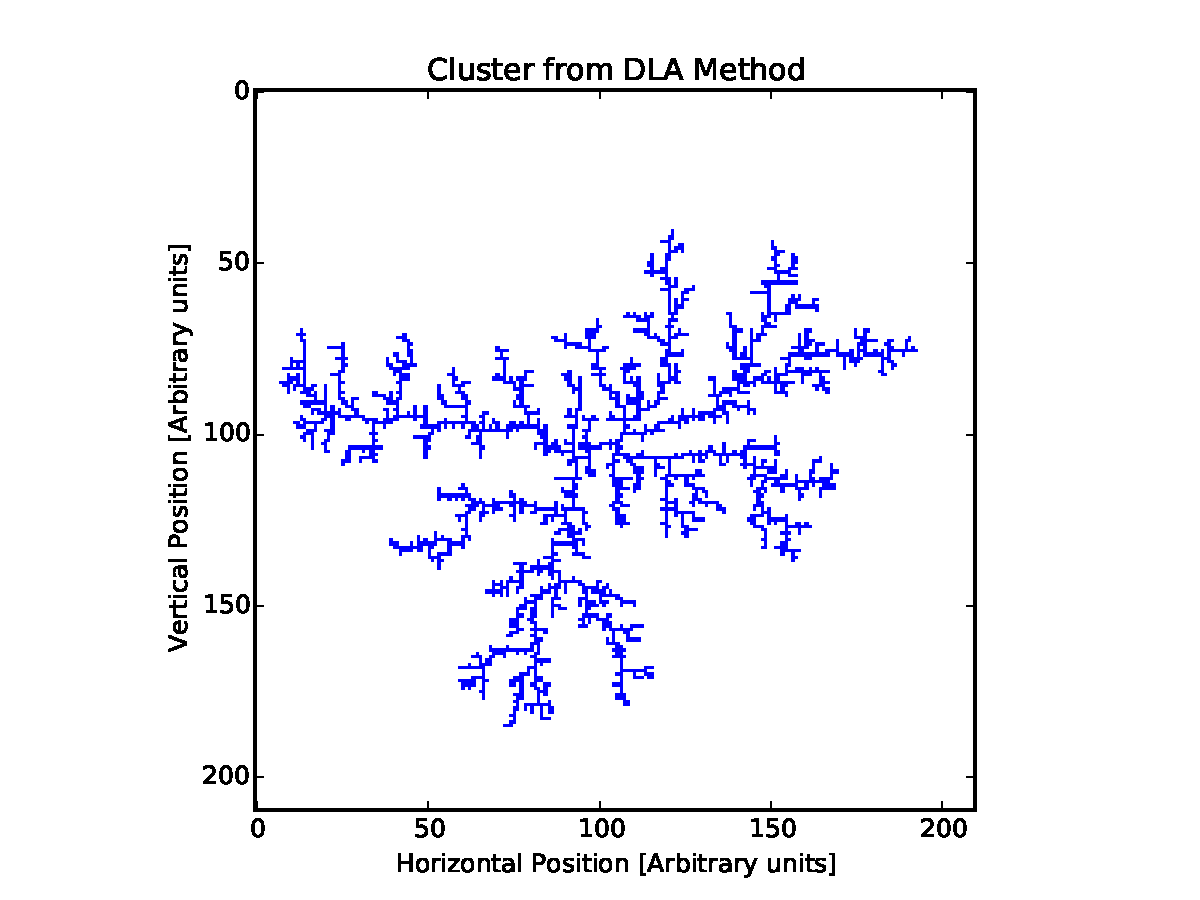
\includegraphics[width = 0.45\textwidth]{pics/DLA_crystal_final_5.pdf} &
		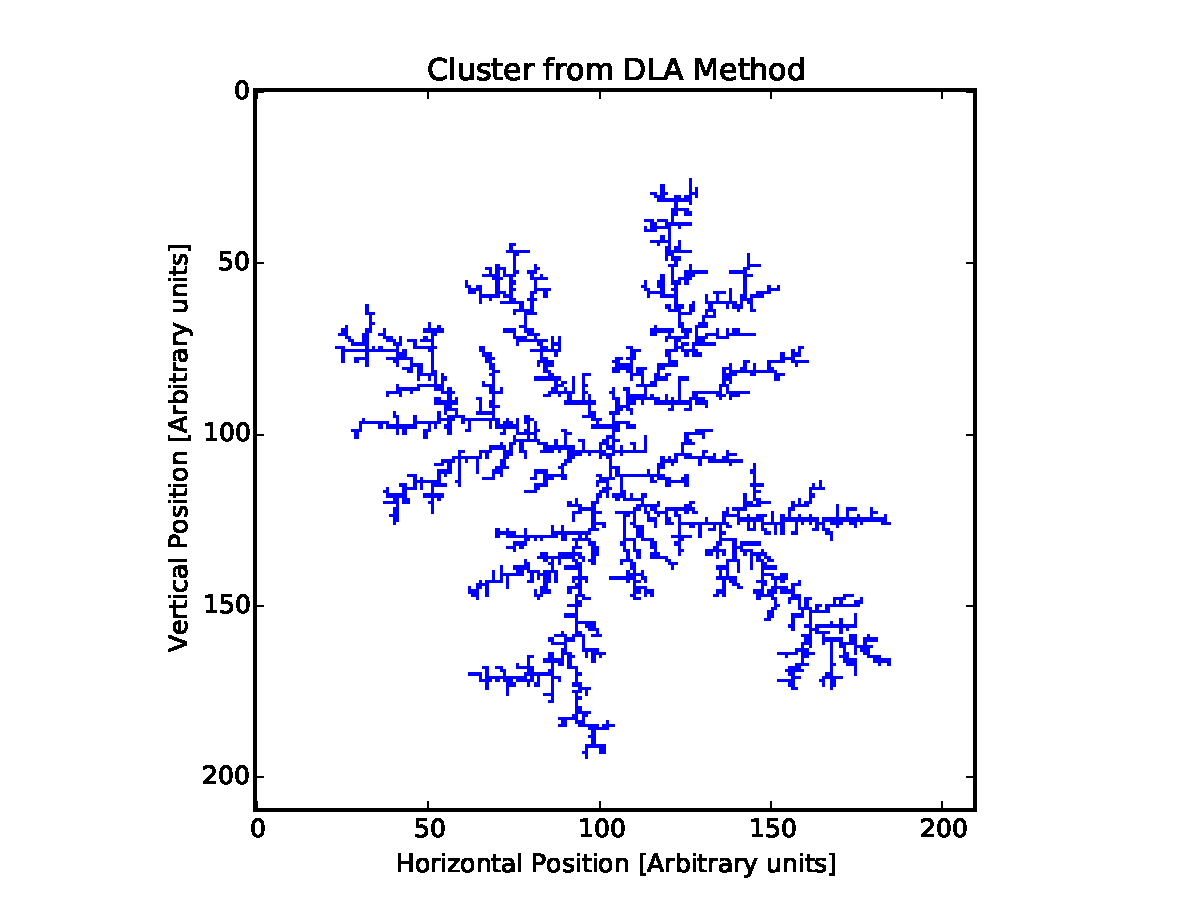
\includegraphics[width = 0.45\textwidth]{pics/DLA_crystal_final_6.pdf} \\
		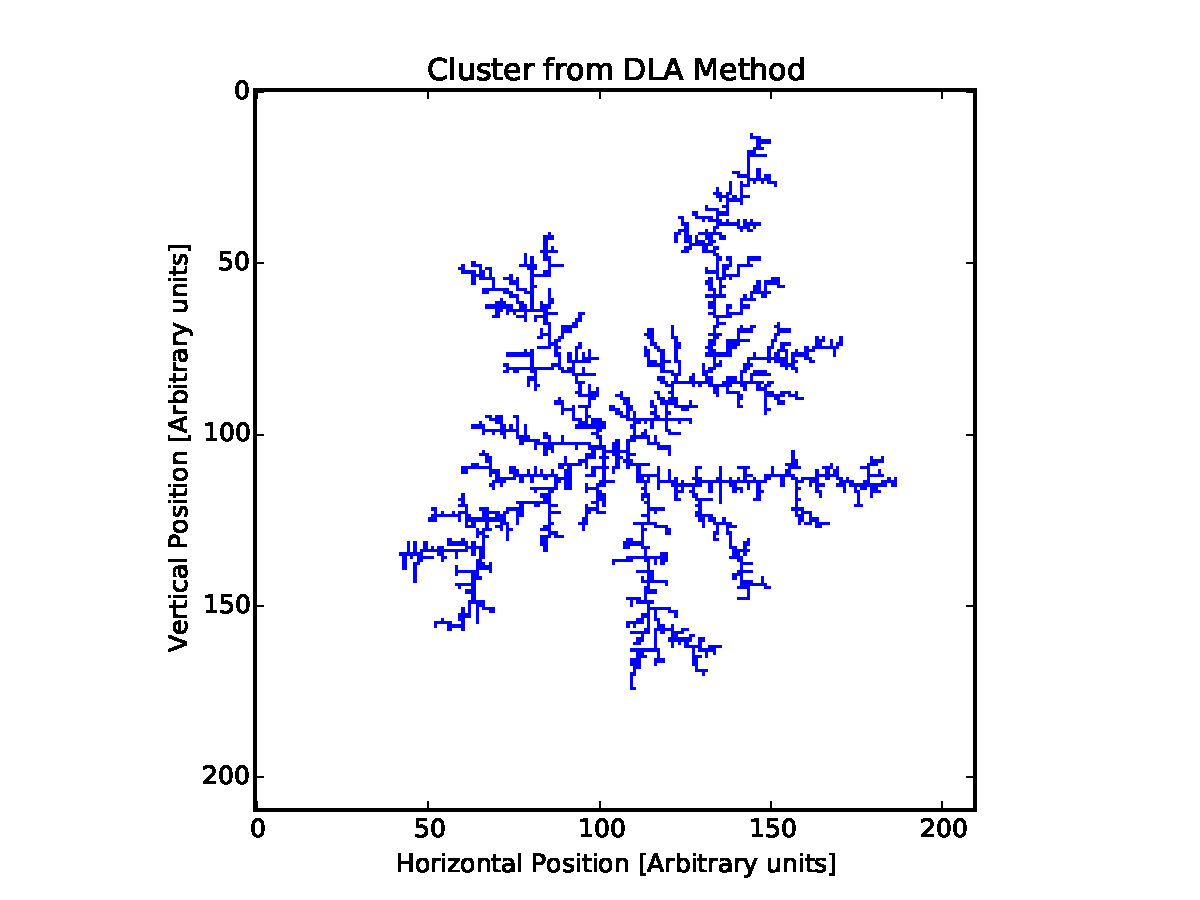
\includegraphics[width = 0.45\textwidth]{pics/DLA_crystal_final_7.pdf} &
		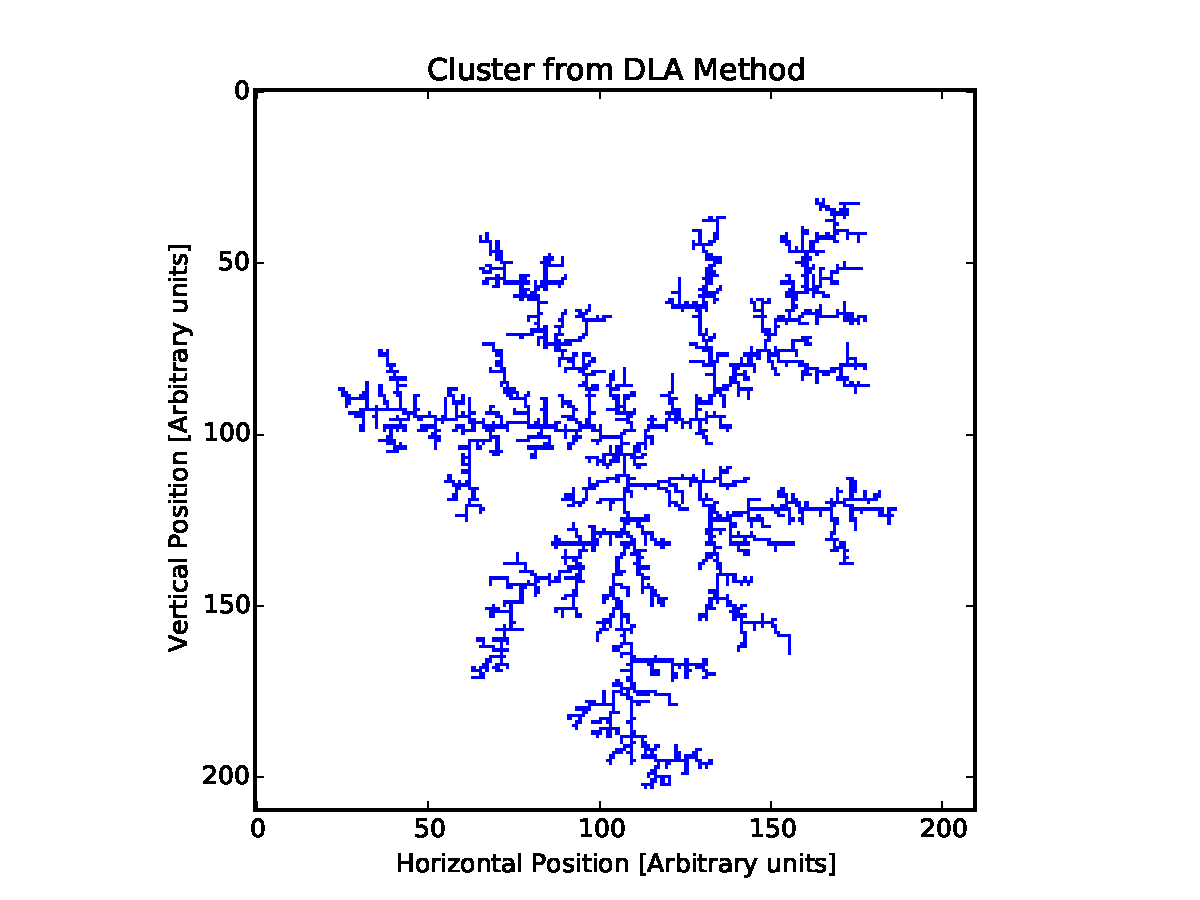
\includegraphics[width = 0.45\textwidth]{pics/DLA_crystal_final_8.pdf} \\
		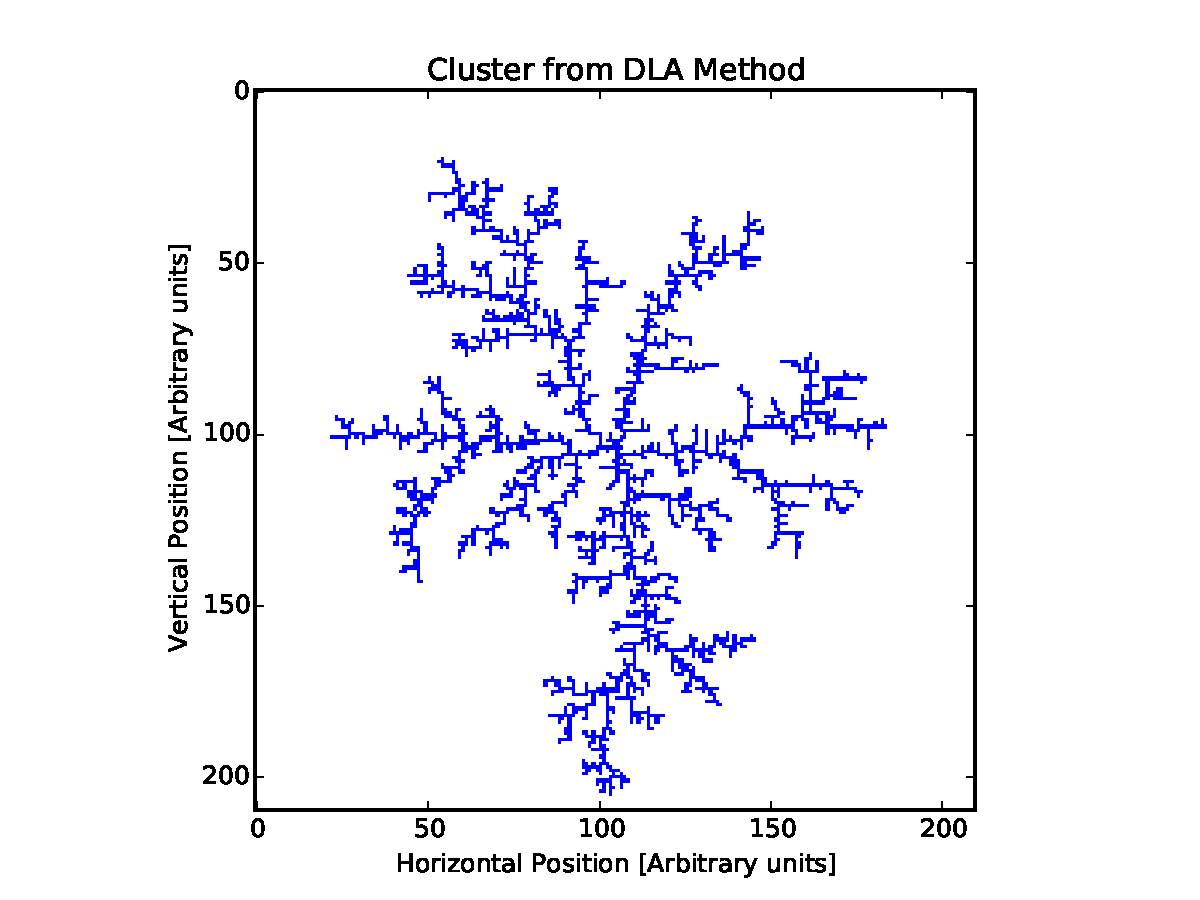
\includegraphics[width = 0.45\textwidth]{pics/DLA_crystal_final_9.pdf} &
		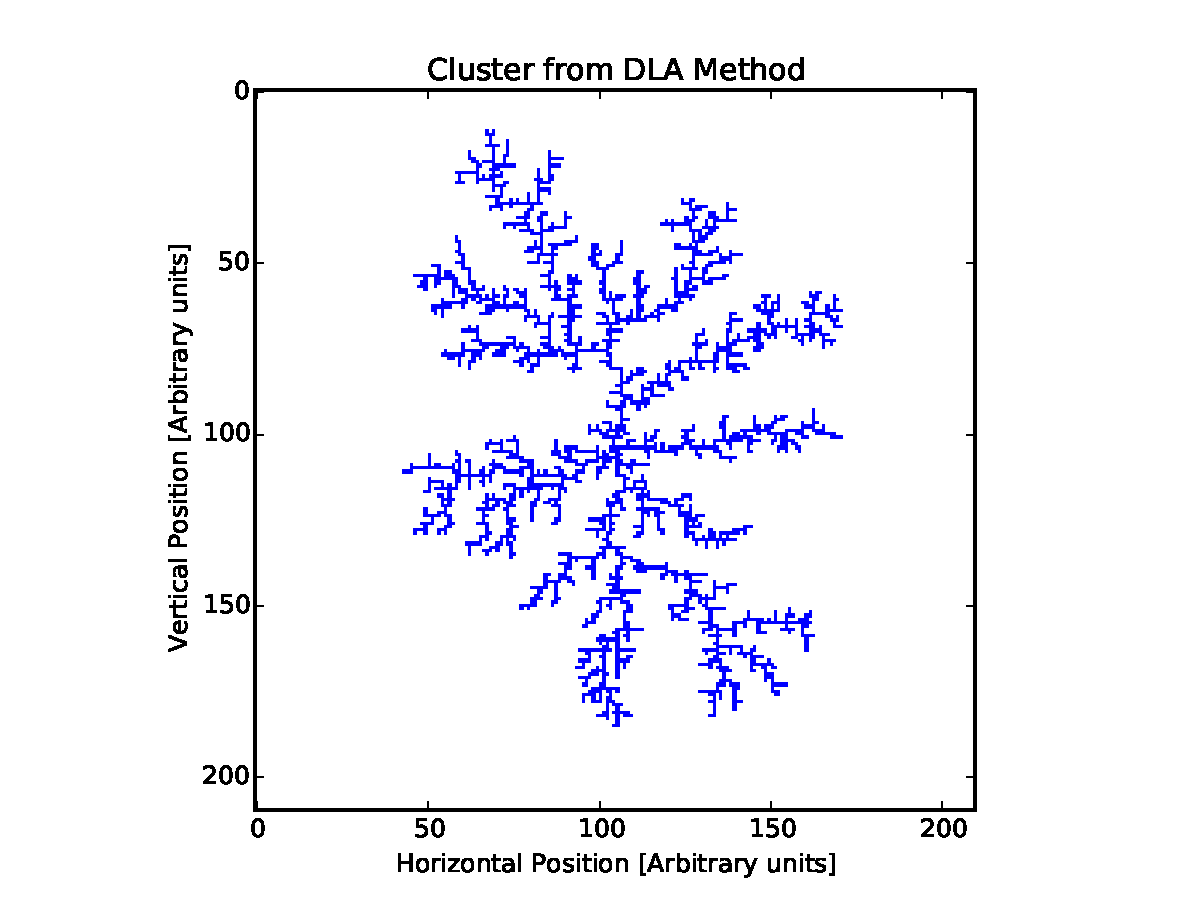
\includegraphics[width = 0.45\textwidth]{pics/DLA_crystal_final_10.pdf} \\
	\end{tabular}
	\caption{DLA cluster: Trial 1 to 10. The average number of walkers used was ....with a standard deviation of $\pm...$}
	\label{DLAcluster}
\end{figure}


\indent The fractal dimension is a parameter that gives the distribution of "mass" of number of walkers in the cluster, as a function of radius
\begin{equation}
m = C*r^df $$\\$$
\log{m} = C + df*\log{r} $$\\$$
\label{fractal dimension}
\end{equation}
Where, \\
m = mass or the number of walkers (each walker is given a unit mass);\\
C = constant of proportionality; \\
r = radius of cluster; \\
df = fractal dimension of cluster \\

\indent When the log-log plot of mass Vs radius is plotted it comes to be a straight line, with the slope of the line giving the fractal dimension nd the y intercept giving the constant. 
A total of ten iterations were done to get ten clusters, and for each cluster, a log-log plot showing the distribution of mass with respect to radius, was generated. For greater accuracy in the fractal dimensionality
calculations, the masses of the ten clusters were averaged for each radius value, and another log-log plot of the mass distribution was generated.

\begin{figure}[htb]
\centering
	\begin{tabular}{@{}cc@{}}
		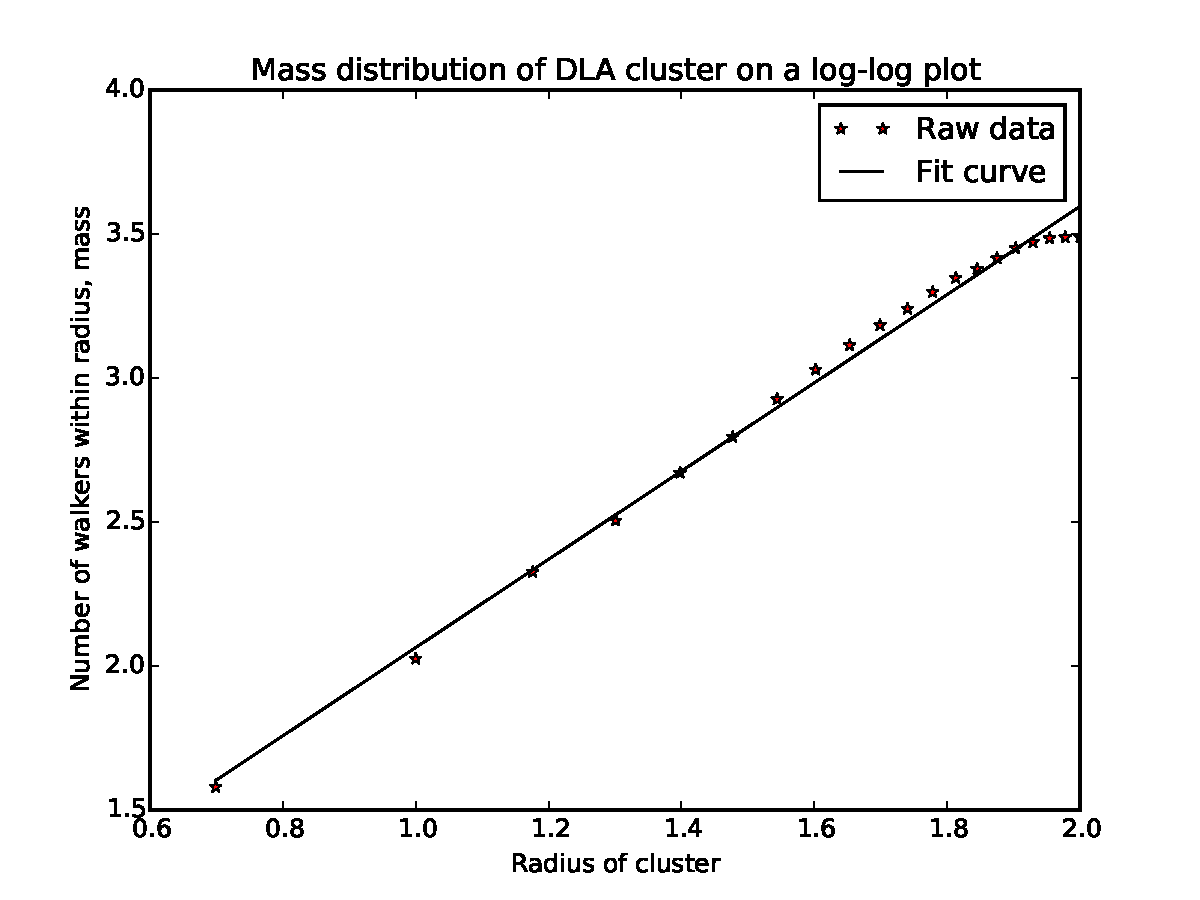
\includegraphics[width = 0.45\textwidth]{pics/Fractal_dimension_final_1.pdf} &
		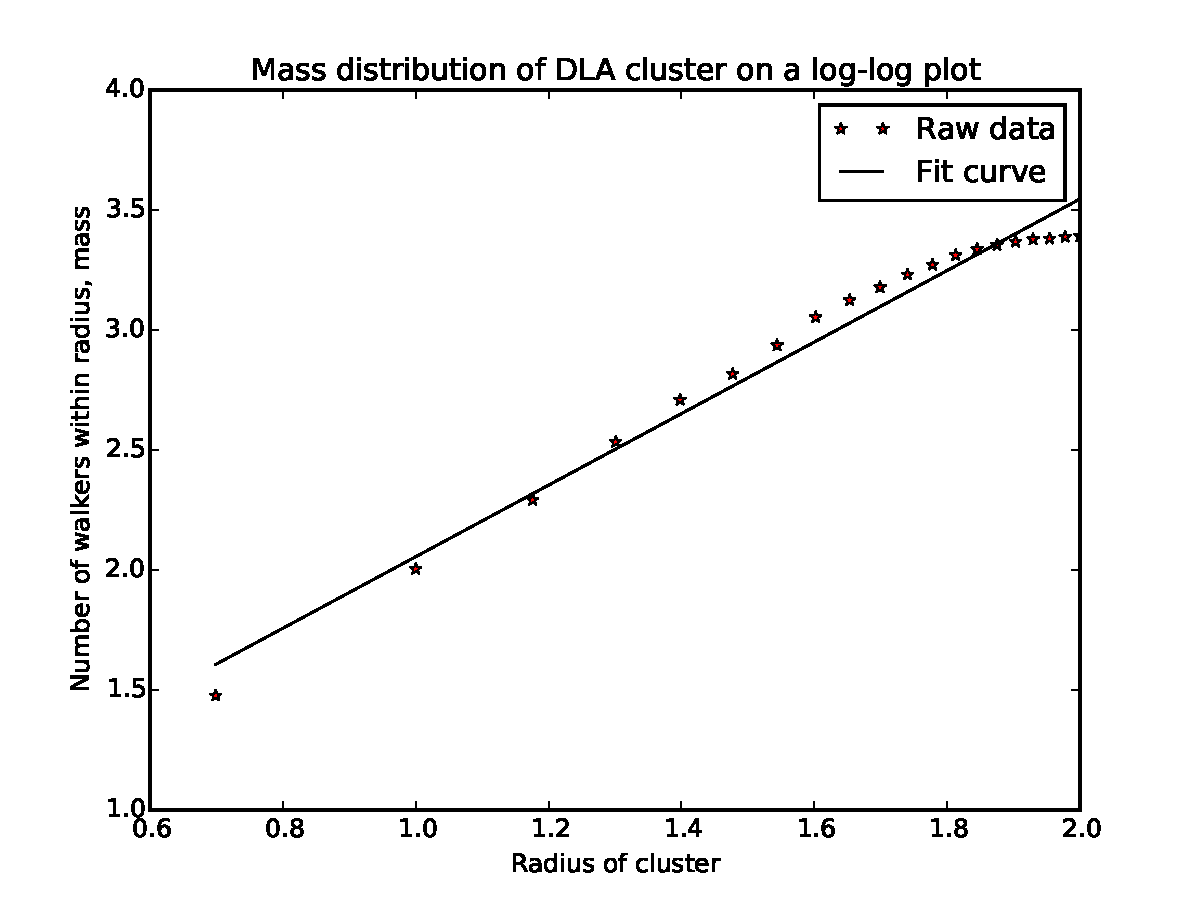
\includegraphics[width = 0.45\textwidth]{pics/Fractal_dimension_final_2.pdf} \\
		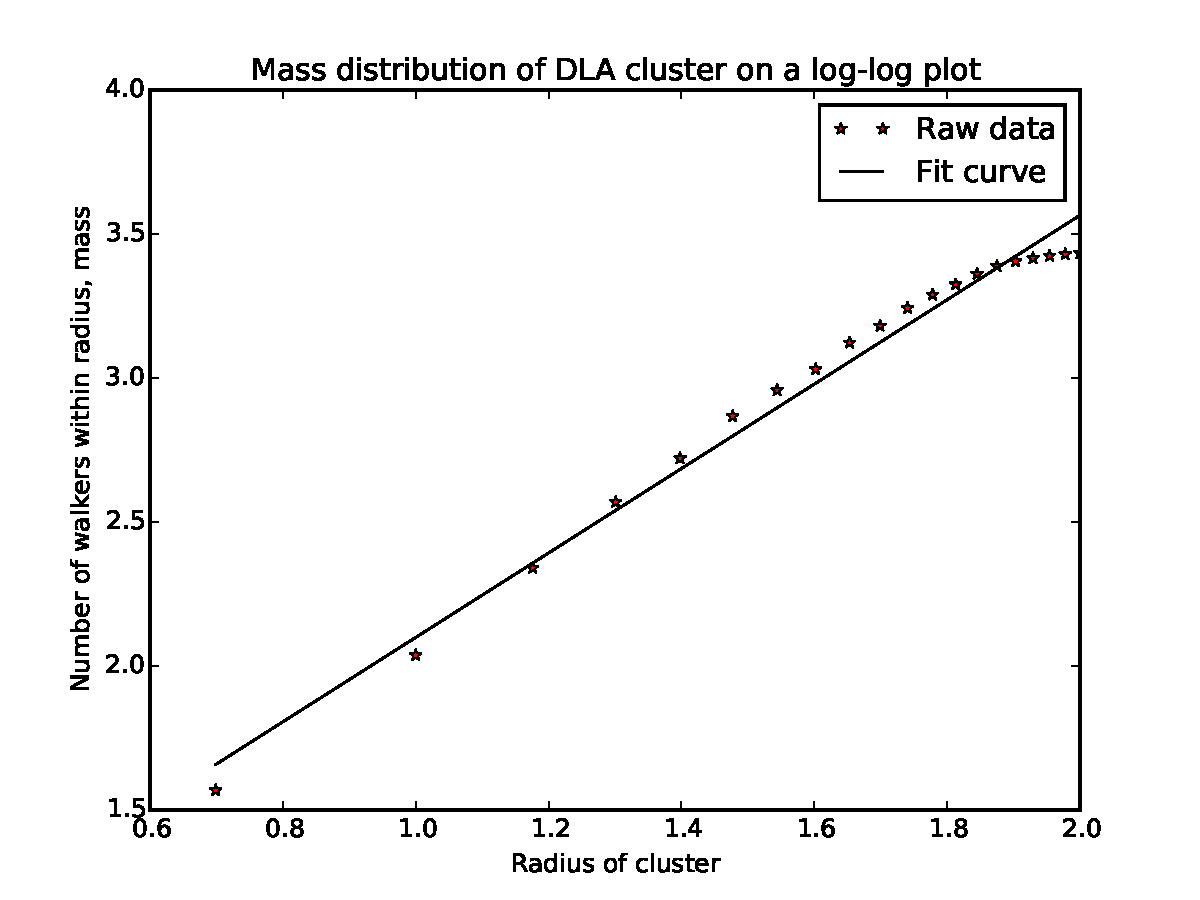
\includegraphics[width = 0.45\textwidth]{pics/Fractal_dimension_final_3.pdf} &
		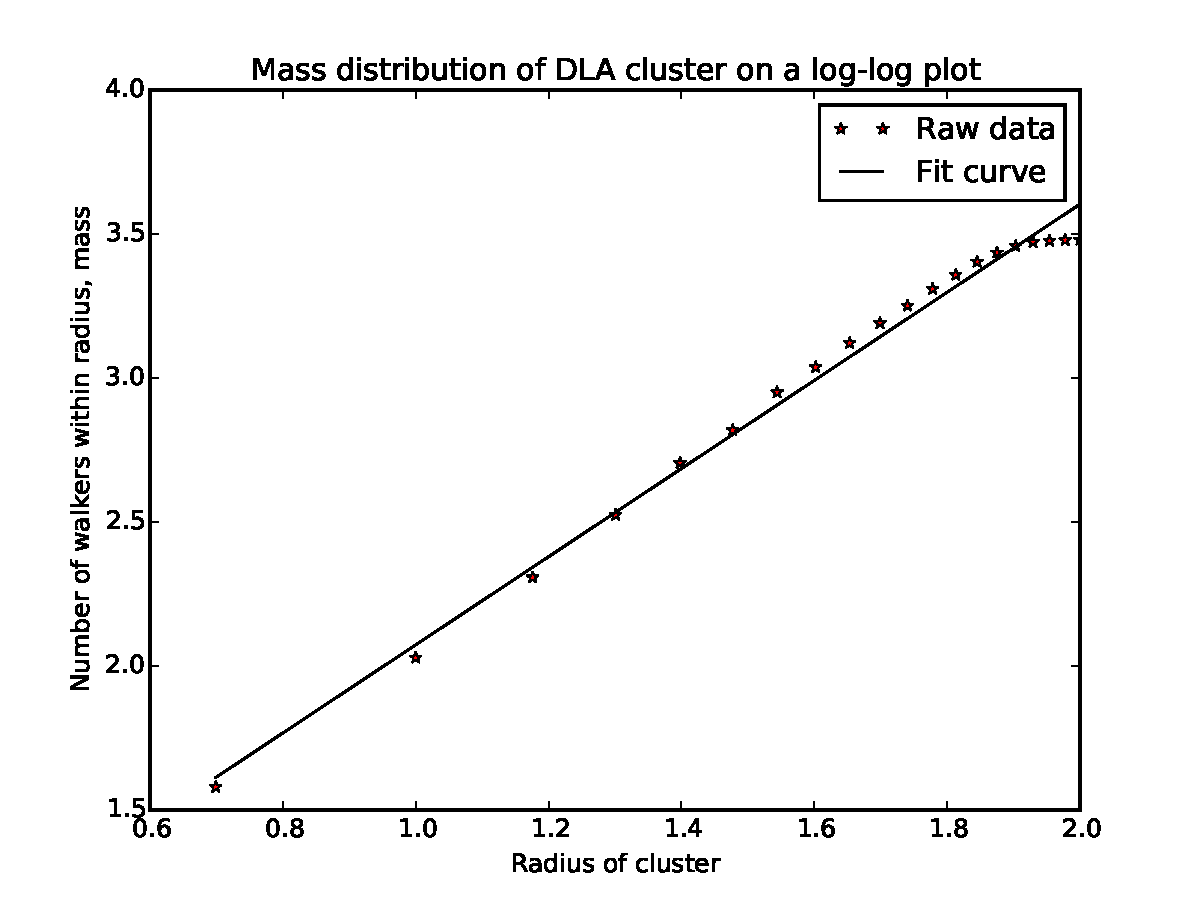
\includegraphics[width = 0.45\textwidth]{pics/Fractal_dimension_final_4.pdf} \\
		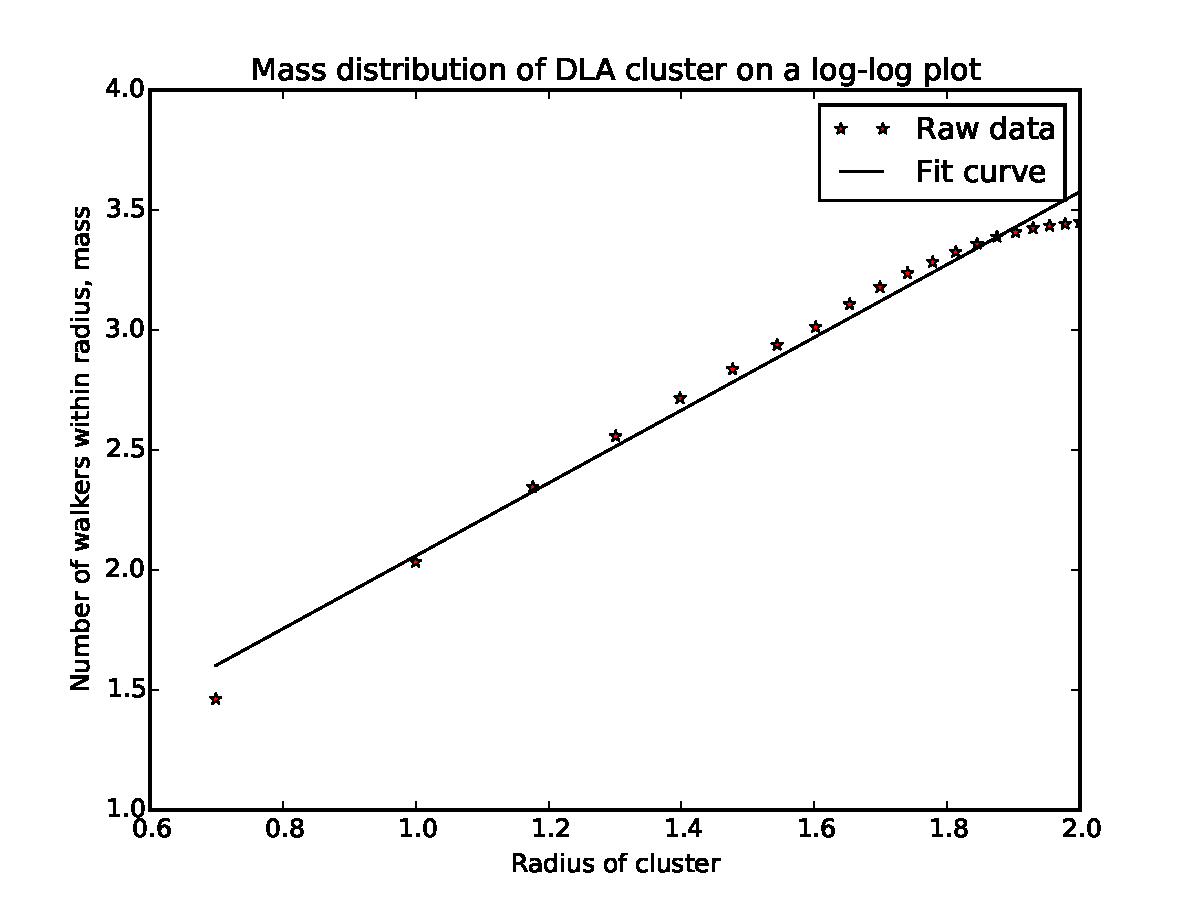
\includegraphics[width = 0.45\textwidth]{pics/Fractal_dimension_final_5.pdf} &
		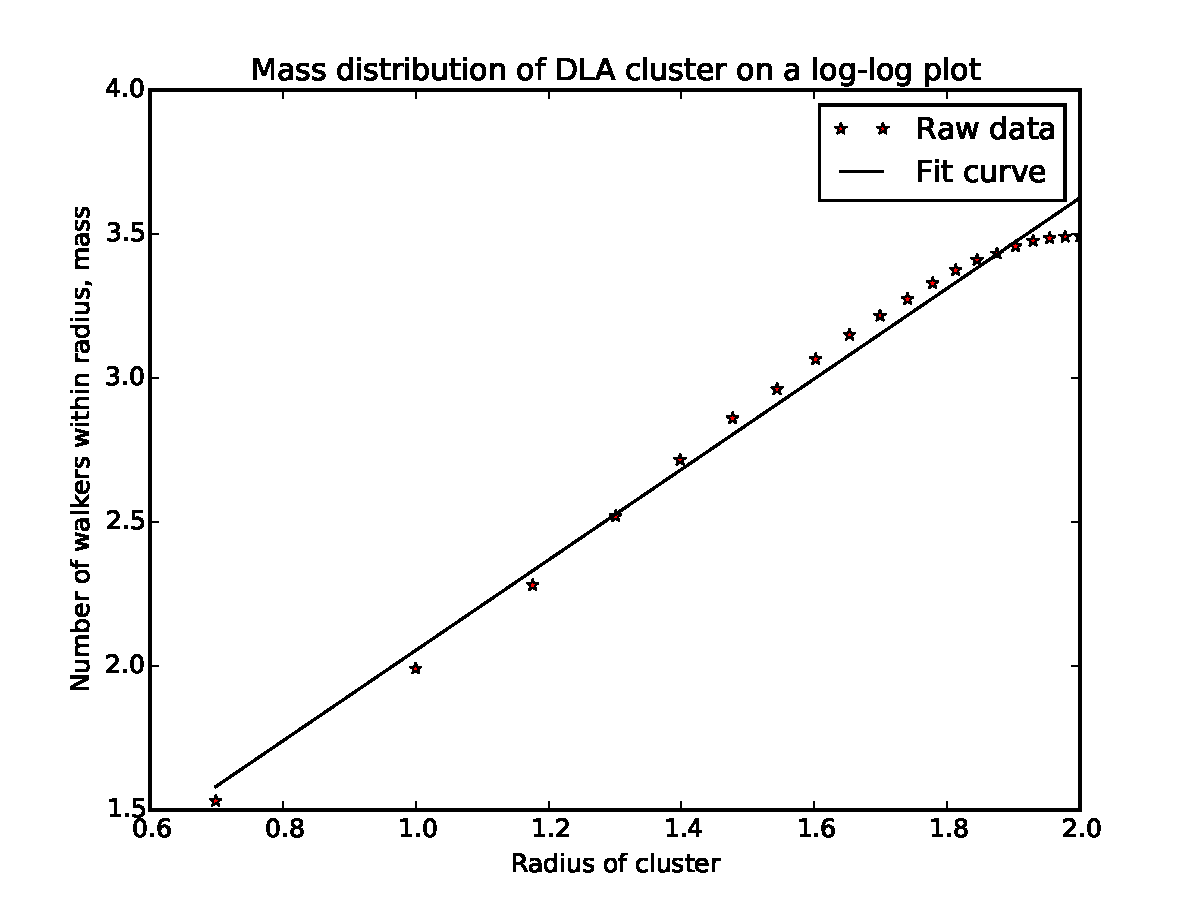
\includegraphics[width = 0.45\textwidth]{pics/Fractal_dimension_final_6.pdf} \\
		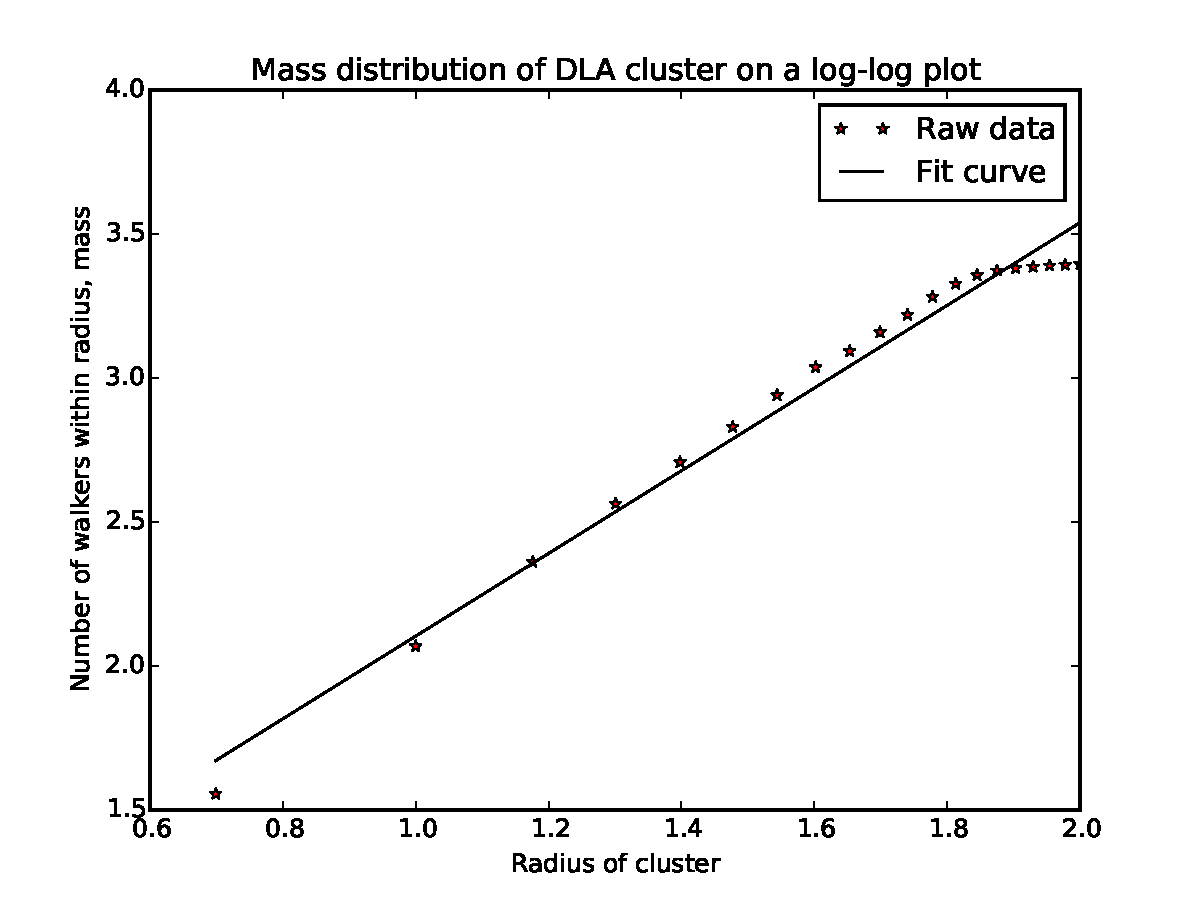
\includegraphics[width = 0.45\textwidth]{pics/Fractal_dimension_final_7.pdf} &
		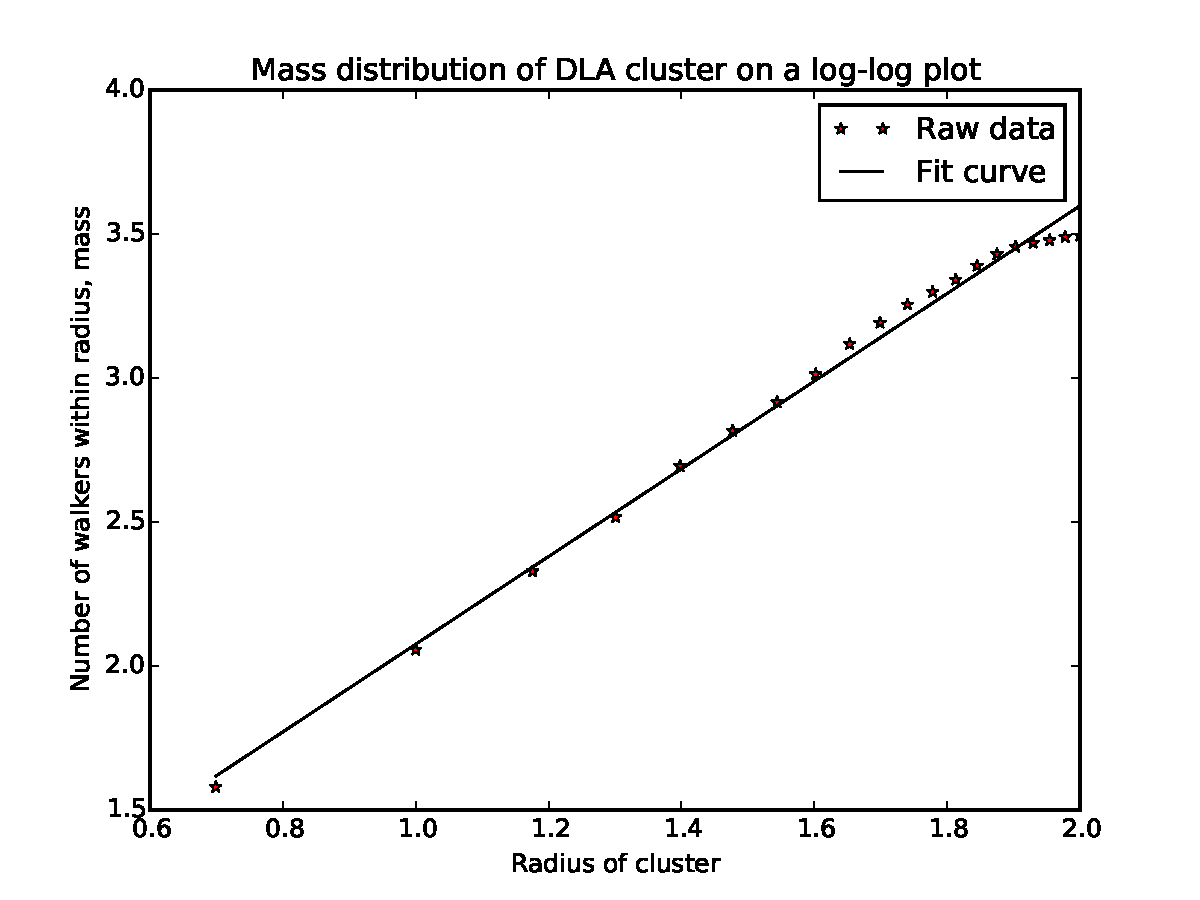
\includegraphics[width = 0.45\textwidth]{pics/Fractal_dimension_final_8.pdf} \\
		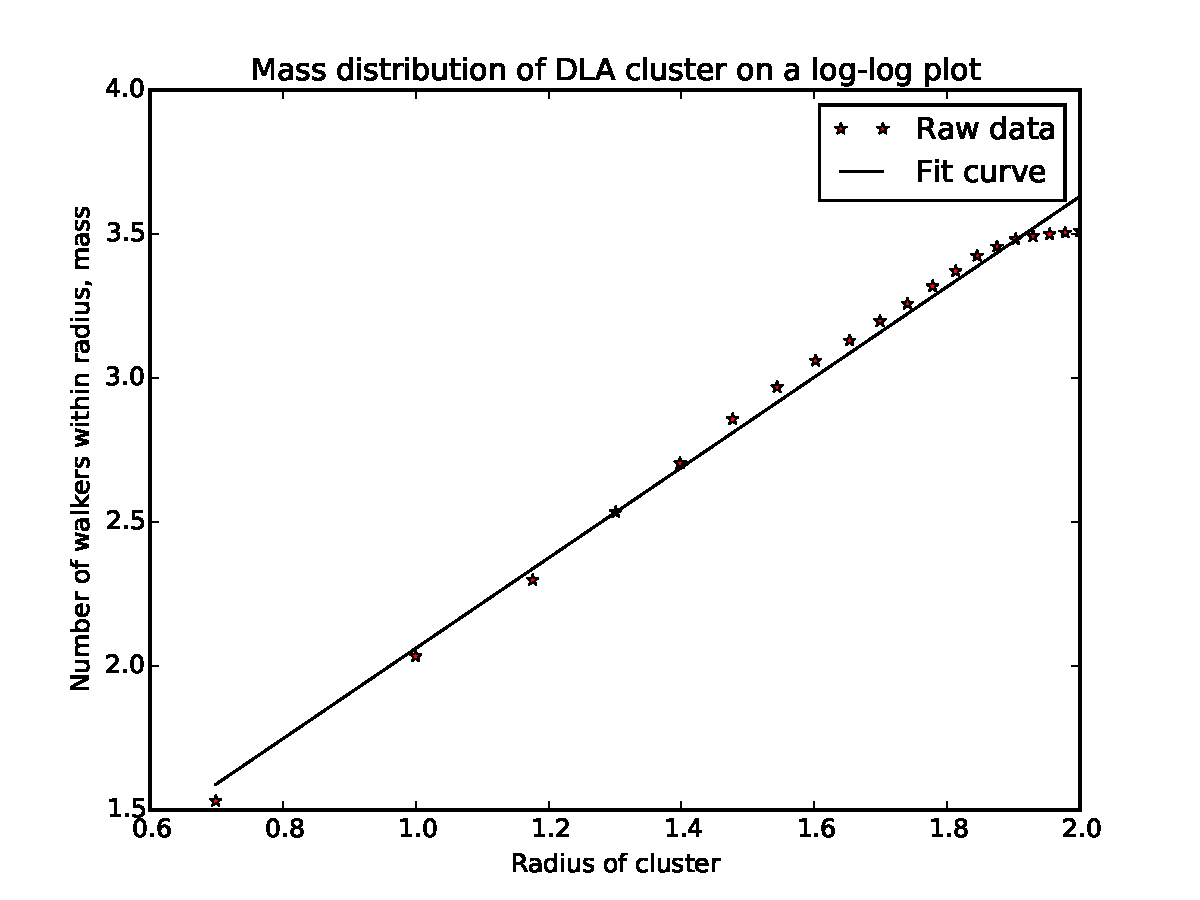
\includegraphics[width = 0.45\textwidth]{pics/Fractal_dimension_final_9.pdf} &
		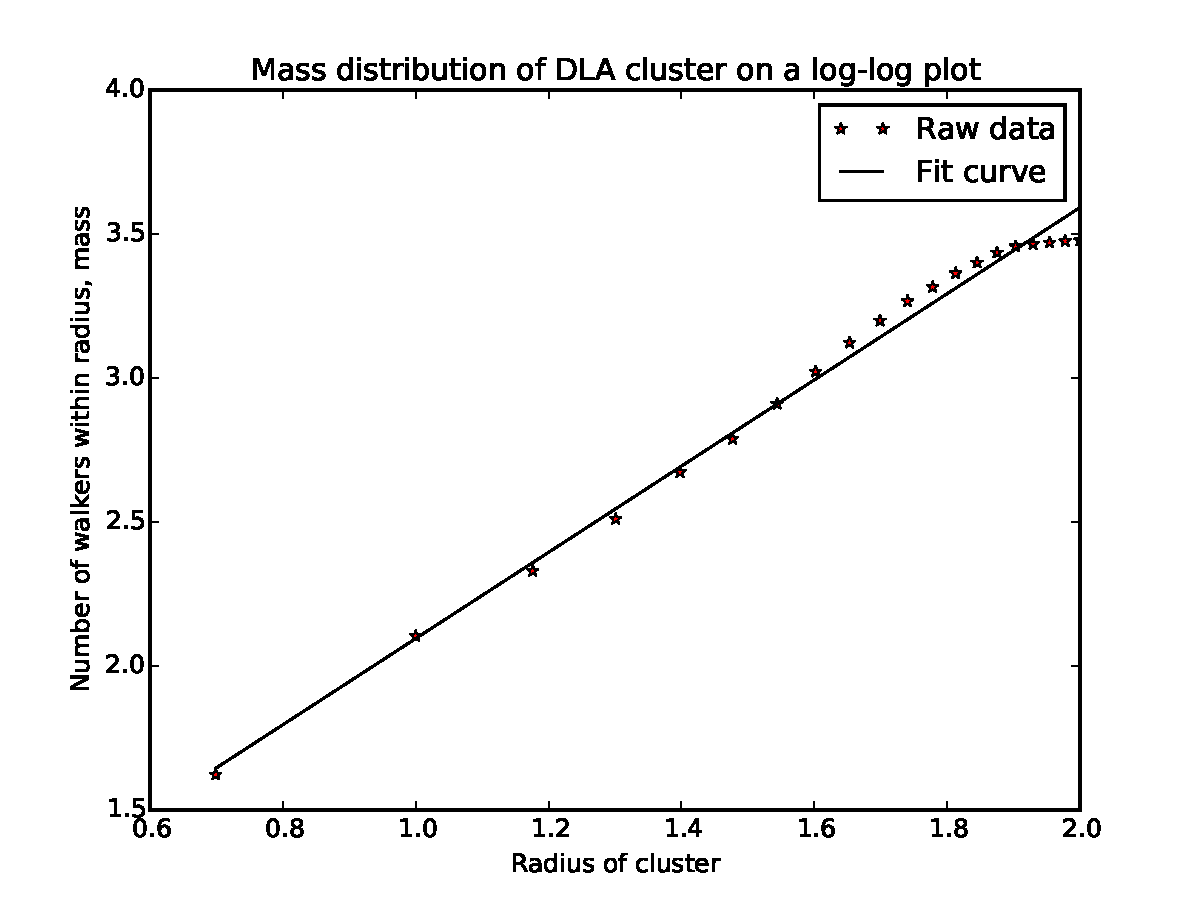
\includegraphics[width = 0.45\textwidth]{pics/Fractal_dimension_final_10.pdf} \\
	\end{tabular}
	\caption{Mass distribution w.r.t radius: Trial 1 to 10. The average fractal dimension was .... with a standard deviation of $\pm...$}
	\label{FractalDimension}
\end{figure}

\begin{figure}[htbp]
\begin{center}
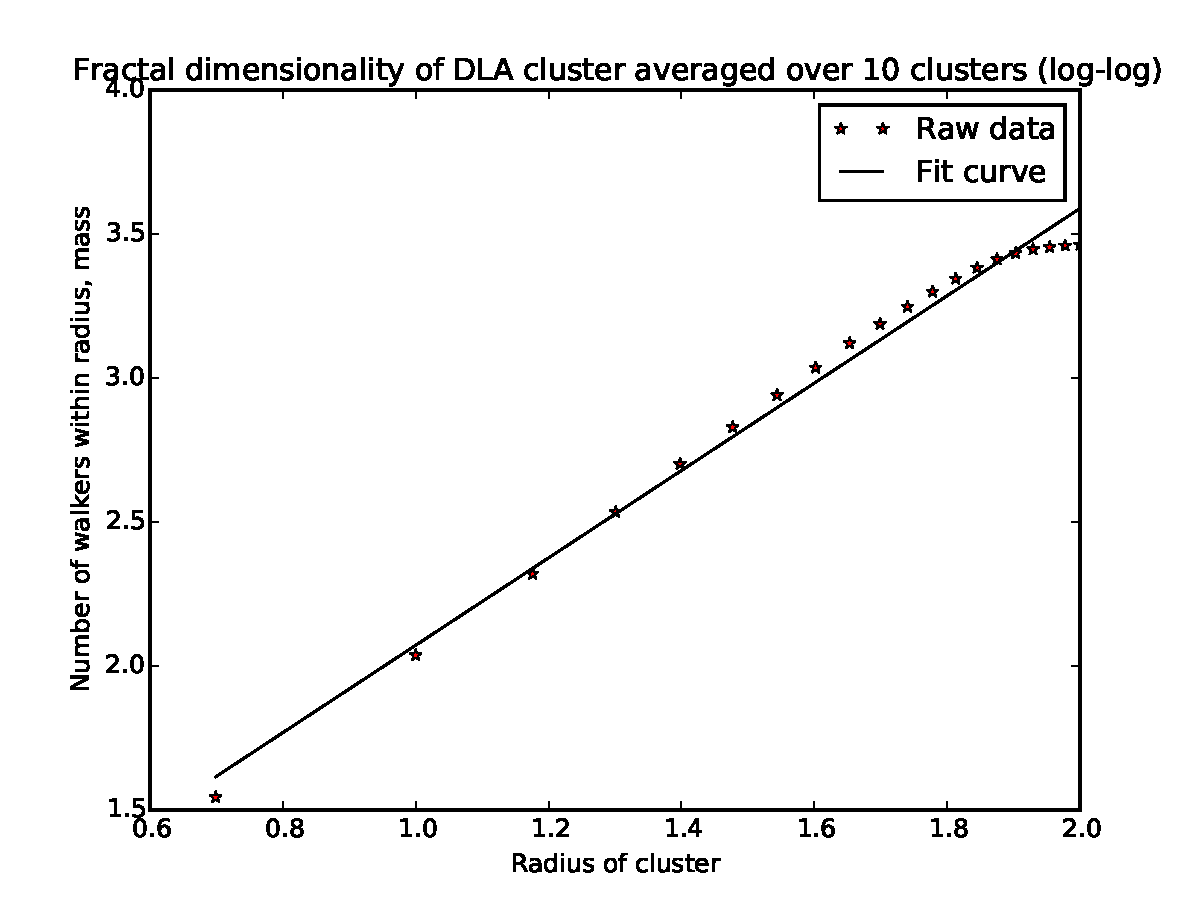
\includegraphics[width = \textwidth]{pics/Fractal_dimension_final_avg.pdf}
\caption{The average mass over ten trials of cluster growth at different radii. The slope gives the average fractal dimension of the system, which is ...}
\label{AvgFractalDimension}
\end{center}
\end{figure}



\subsection{Results}  
\indent RESULTS TO COME....



\end{document}
